\documentclass[border=4pt]{standalone}
\usepackage{amsmath,amssymb,amsfonts}
\usepackage{xcolor,colortbl,array,booktabs,multirow}
\usepackage{tikz}
\usepackage{pgfplots}
\pgfplotsset{compat=1.16}
\usetikzlibrary{arrows, automata, backgrounds, calendar, chains, decorations,
    matrix, mindmap, patterns, petri, positioning, shadows, shapes.geometric,
    trees, shapes, decorations.pathreplacing, calc, tikzmark, arrows.meta,
    intersections, fit, graphs, quotes, angles, decorations.markings}
\newcommand{\st}{\text{ s.t. }}
\newcommand{\x}{\mathbf{x}}
\renewcommand{\b}{\mathbf{b}}
\renewcommand{\c}{\mathbf{c}}
\newcommand{\A}{\mathbf{A}}
\newcommand{\y}{\mathbf{y}}
\newcommand{\z}{\mathbf{z}}
\newcommand{\R}{\mathbb{R}}
\newcommand{\RR}{\mathbb{R}}
\newcommand{\Z}{\mathbb{Z}}
\newcommand{\ZZ}{\mathbb{Z}}
\newcommand{\npcomplete}{NP-complete}
\providecommand{\true}{\text{TRUE}}
\providecommand{\false}{\text{FALSE}}
\tikzset{vertex/.style={circle,fill=black!25,minimum size=20pt,inner sep=0pt},
    edge/.style={draw,thick,-},weight/.style={font=\small},
    selected vertex/.style={vertex, fill=red!24},
    selected edge/.style={draw,line width=2pt,-,red!50},
    ignored edge/.style={draw,line width=2pt,-,black!20}}
\newcommand{\vect}{\vec}
\providecommand{\ds}{\displaystyle}
\providecommand{\longvect}{\overrightarrow}
\usepackage[normalem]{ulem}
\definecolor{ocre}{RGB}{243,102,25}
\providecommand{\leftB}{\left[}
\providecommand{\rightB}{\right]}
\tikzset{directed/.style={postaction={decorate,decoration={markings,mark=at position .65 with {\arrow{>}}}}},
    directed1/.style={postaction={decorate,decoration={markings,mark=at position .65 with {\arrow{>}}}}}}
\begin{document}
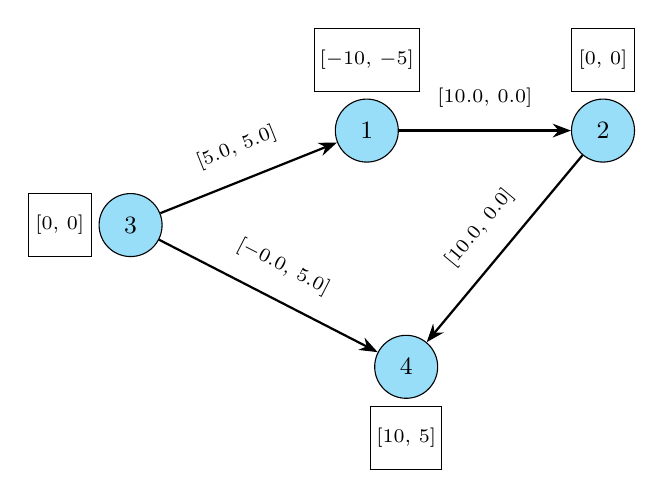
\begin{tikzpicture}[
    every node/.style={circle, draw=black, fill=cyan!40, minimum size=8mm, inner sep=1pt, font=\small},
    every edge/.style={draw, thick},
    >=Stealth,
    node distance=2.5cm and 3cm
  ]
  \node (n1) at (3,3) {1};
  \node (n2) at (6,3) {2};
  \node (n3) at (0,1.8) {3};
  \node (n4) at (3.5,0) {4};

  % Supply/demand annotations
  \node[draw=black, fill=white, rectangle, font=\scriptsize, inner sep=2pt] at (3,3.9) {$[-10,\,-5]$};
  \node[draw=black, fill=white, rectangle, font=\scriptsize, inner sep=2pt] at (6,3.9) {$[0,\,0]$};
  \node[draw=black, fill=white, rectangle, font=\scriptsize, inner sep=2pt] at (-0.9,1.8) {$[0,\,0]$};
  \node[draw=black, fill=white, rectangle, font=\scriptsize, inner sep=2pt] at (3.5,-0.9) {$[10,\,5]$};

  % Arcs with optimal commodity flows [f_{ij1}, f_{ij2}]
  \draw[->, thick] (n3) -- (n1) node[midway, sloped, above, font=\scriptsize, fill=none, draw=none, rectangle] {$[5.0,\,5.0]$};
  \draw[->, thick] (n1) -- (n2) node[midway, above, font=\scriptsize, fill=none, draw=none, rectangle] {$[10.0,\,0.0]$};
  \draw[->, thick] (n2) -- (n4) node[midway, sloped, above, font=\scriptsize, fill=none, draw=none, rectangle] {$[10.0,\,0.0]$};
  \draw[->, thick] (n3) -- (n4) node[midway, sloped, above, font=\scriptsize, fill=none, draw=none, rectangle] {$[-0.0,\,5.0]$};
\end{tikzpicture}
\end{document}
